\documentclass[12pt]{article}
\usepackage[]{color}

%% maxwidth is the original width if it is less than linewidth
%% otherwise use linewidth (to make sure the graphics do not exceed the margin)
\makeatletter
\def\maxwidth{ %
	\ifdim\Gin@nat@width>\linewidth
	\linewidth
	\else
	\Gin@nat@width
	\fi
}
\makeatother

\definecolor{fgcolor}{rgb}{0.345, 0.345, 0.345}
\newcommand{\hlnum}[1]{\textcolor[rgb]{0.686,0.059,0.569}{#1}}%
\newcommand{\hlstr}[1]{\textcolor[rgb]{0.192,0.494,0.8}{#1}}%
\newcommand{\hlcom}[1]{\textcolor[rgb]{0.678,0.584,0.686}{\textit{#1}}}%
\newcommand{\hlopt}[1]{\textcolor[rgb]{0,0,0}{#1}}%
\newcommand{\hlstd}[1]{\textcolor[rgb]{0.345,0.345,0.345}{#1}}%
\newcommand{\hlkwa}[1]{\textcolor[rgb]{0.161,0.373,0.58}{\textbf{#1}}}%
\newcommand{\hlkwb}[1]{\textcolor[rgb]{0.69,0.353,0.396}{#1}}%
\newcommand{\hlkwc}[1]{\textcolor[rgb]{0.333,0.667,0.333}{#1}}%
\newcommand{\hlkwd}[1]{\textcolor[rgb]{0.7te37,0.353,0.396}{\textbf{#1}}}%

%\usepackage{framed}
%\makeatletter
%\newenvironment{kframe}{%
%	\def\at@end@of@kframe{}%
%	\ifinner\ifhmode%
%	\def\at@end@of@kframe{\end{minipage}}%
%\begin{minipage}{\columnwidth}%
%	\fi\fi%
%	\def\FrameCommand##1{\hskip\@totalleftmargin \hskip-\fboxsep
%		\colorbox{shadecolor}{##1}\hskip-\fboxsep
%		% There is no \\@totalrightmargin, so:
%		\hskip-\linewidth \hskip-\@totalleftmargin \hskip\columnwidth}%
%	\MakeFramed {\advance\hsize-\width
%		\@totalleftmargin\z@ \linewidth\hsize
%		\@setminipage}}%
%{\par\unskip\endMakeFramed%
%	\at@end@of@kframe}
%\makeatother

\definecolor{shadecolor}{rgb}{.97, .97, .97}
\definecolor{messagecolor}{rgb}{0, 0, 0}
\definecolor{warningcolor}{rgb}{1, 0, 1}
\definecolor{errorcolor}{rgb}{1, 0, 0}
\newenvironment{knitrout}{}{} % an empty environment to be redefined in TeX

%%% FONT AND INPUT
\usepackage[T5]{fontenc}
\usepackage[utf8]{inputenc} % set input encoding (not needed with XeLaTeX)

%%% Examples of Article customizations
% These packages are optional, depending whether you want the features they provide.
% See the LaTeX Companion or other references for full information.

%%% PAGE DIMENSIONS
\usepackage{geometry} % to change the page dimensions
\geometry{letterpaper} % or letterpaper (US) or a5paper or....
\geometry{margin=1in} % for example, change the margins to 2 inches all round
% \geometry{landscape} % set up the page for landscape
%   read geometry.pdf for detailed page layout information

\usepackage{graphicx} % support the \includegraphics command and options

% \usepackage[parfill]{parskip} % Activate to begin paragraphs with an empty line rather than an indent

%%% PACKAGES
\usepackage{booktabs} % for much better looking tables
\usepackage{array} % for better arrays (eg matrices) in maths
\usepackage{paralist} % very flexible & customisable lists (eg. enumerate/itemize, etc.)
\usepackage{verbatim} % adds environment for commenting out blocks of text & for better verbatim
\usepackage{subcaption} % make it possible to include more than one captioned figure/table in a single float
\usepackage{float}
\usepackage{setspace}
\usepackage{amsmath,newtxtext,newtxmath}
\usepackage{url}
\usepackage{multirow}
\usepackage{listings}
\usepackage{dcolumn}
%\usepackage[nolists]{endfloat}
\usepackage{bbm}
\usepackage{pdflscape}
\usepackage{pdfpages}
\usepackage{tikz} 
\usetikzlibrary{arrows,decorations.pathmorphing,decorations.pathreplacing,backgrounds,fit,positioning,shapes.symbols,chains}

%%% HEADERS & FOOTERS
\usepackage{fancyhdr} % This should be set AFTER setting up the page geometry
\pagestyle{fancy} % options: empty , plain , fancy
\renewcommand{\headrulewidth}{0pt} % customise the layout...
\lhead{}\chead{}\rhead{}
\lfoot{}\cfoot{\thepage}\rfoot{}

%%% CITATION AND BIBLIOGRAPHY

\usepackage[authordate,backend=bibtex8,natbib,sorting=nyt,sortcites,isbn=false,doi=false]{biblatex-chicago}
%\usepackage{natbib}
%\bibliographystyle{apsr}
\bibliography{Literature/library_syp}

% fix problem with \citeyear and \citeyearpar not being highlighted
\DeclareCiteCommand{\citeyear}
	{}
	{\bibhyperref{\printdate}}
	{\multicitedelim}
	{}

\DeclareCiteCommand{\citeyearpar}
	{}
	{\mkbibparens{\bibhyperref{\printdate}}}
	{\multicitedelim}
	{}
% possessive cite with \citepos
\newcommand\citepos[1]{\citeauthor{#1}'s\ (\citeyear{#1})}

% change fnote style to normal text, double-spaced
\renewcommand{\footnotesize}{\normalsize}
\newcommand\fnote[1]{\footnote{\baselineskip=2\normalbaselineskip#1}}
\setlength{\footnotesep}{2pc}

\usepackage{hyperref}
\hypersetup{
	colorlinks=true,
	linkcolor=blue,
	filecolor=magenta,      
	urlcolor=cyan,
}

%%% SECTION TITLE APPEARANCE
\usepackage{sectsty}
%\allsectionsfont{\sffamily\mdseries\upshape} % (See the fntguide.pdf for font help)
% (This matches ConTeXt defaults)

%%% ToC (table of contents) APPEARANCE
\usepackage[nottoc,notlof,notlot]{tocbibind} % Put the bibliography in the ToC
\usepackage[titles,subfigure]{tocloft} % Alter the style of the Table of Contents
\renewcommand{\cftsecfont}{\rmfamily\mdseries\upshape}
\renewcommand{\cftsecpagefont}{\rmfamily\mdseries\upshape} % No bold!

%%% Some commands
\newcommand{\reg}{\texttt{regress} }
\newcommand{\1}{\mathbbm{1}}

\renewcommand\r{\right}
\renewcommand\l{\left}
\newcommand\E{\mathbbm{E}}
\newcommand\V{\mathbbm{V}}
\newcommand\Var{\mathbbm{V}}
\newcommand\avar{{\rm Avar}}
\newcommand\dist{\buildrel\rm d\over\sim}
\newcommand\iid{\stackrel{\rm i.i.d.}{\sim}}
\newcommand\ind{\stackrel{\rm indep.}{\sim}}
\newcommand\cov{{\rm Cov}}
\newcommand{\R}{\textbf{R} }
\newcommand{\Rcmd}[1]{{\large \texttt{#1}}}
\newcommand\indep{\protect\mathpalette{\protect\independenT}{\perp}}
\def\independenT#1#2{\mathrel{\rlap{$#1#2$}\mkern2mu{#1#2}}}
\DeclareMathOperator{\sgn}{sgn}
\DeclareMathOperator*{\argmin}{argmin}

\newcommand\Sum{\sum^N_{i=1}}
\newcommand\Prod{\prod^N_{i=1}}
\newcommand{\pderiv}[1]{\frac{\partial}{\partial #1}}
\newcommand{\B}[1]{\boldsymbol{#1}}
\newcommand{\logit}{\text{logit}}

%%% texcount
% Run texcount on tex-file and write results to a sum-file
\immediate\write18{texcount  \jobname.tex -out=\jobname.sum -incbib -relaxed}
% Define macro \wordcount for including the counts
\newcommand\wordcount{\verbatiminput{\jobname.sum}}


%opening
\title{Tea Leaf Elections: \\
	Inferring Purpose for Authoritarian Elections from Post-election Responses to Defeats}
%\author{Minh Trinh}
\date{July 31, 2019}

\begin{document}
	
%TC:ignore 

\maketitle
\thispagestyle{empty}
\doublespacing

\begin{abstract}
The power of authoritarian elections is not unlimited. When using elections as a source of information, dictators may not be able to collect from a single election all the information it could theoretically provide, and so must judiciously decide which specific signal to seek. It is possible to identify the type of information each regime seeks from its elections by studying its reactions to small but unexpected defeats. Applying this logic to the case of Vietnam, I find that the ruling Communist Party of Vietnam responded to the defeats of its favored candidates in the 2016 election for the national legislature by increasing central transfers to provinces where it suffered these defeats. This evidence suggests that the Party uses elections as an opinion poll to identify areas it is less popular in, instead of as an evaluation device to identify local leaders who under-perform in their electoral mobilization efforts.
\end{abstract}

Word count: 9960

%TC:endignore 

\newpage
\pagenumbering{arabic}

\section{Introduction}

At first glance, authoritarian elections seem to be an all-powerful weapon in the dictator's arsenal: not only do they rarely pose existential threats, these elections also serve to cement autocrats' rule by providing critical information on many variables otherwise unknowable, alerting regime rulers to potential threats both internal and external, or simply updating them about the moods and preferences of the public. The literature that discusses authoritarian elections' many informational functions, however, has not considered potential conflict between them. Specifically, an election that is designed to provide information on some aspects of governance and social control may become less effective at shedding light on some others. This forces authoritarian rulers to set priorities and use elections as a telescope focused on a few areas of interest, rather than a panoramic camera that captures every information that comes into view.

Using the case of Vietnam, I show that the Communist Party of Vietnam (CPV) needs information on both the sub-national distribution of regime support and on the quality of its local officials, but uses elections to shed light only on the former. Specifically, I take advantage of rare and unexpected defeats by regime-favored candidates in Vietnam's 2016 legislative election, defeats that the regime did not want to suffer, but still did not do everything it could to avoid. Using three different empirical methods, I show that the CPV increased central transfers from Hanoi to provinces it has suffered defeats in. This finding is consistent with the hypothesis that the regime saw these defeats as indicators for pockets of disillusioned citizens and spent money to placate them. It also rejects the hypothesis that the regime used election defeats to identify provinces with under-performing local officials. Under this alternative hypothesis the CPV would have wanted to punish officials in these provinces, but the increased central transfers would have accomplished only the opposite.

Using detailed empirical evidence from the case of Vietnam, this paper contributes to the larger literature on authoritarian elections. Its main theoretical contribution is to demonstrate how existing theories about authoritarian elections' functionality may not all apply to some certain cases -- specifically those that portray elections as the autocrat's opinion poll \citep[e.g.][]{Miller2015, Magaloni2006, Blaydes2010} and those that portray them as a test to evaluate regime agents \citep[e.g.][]{Magaloni2006, Blaydes2010,Myagkov2009,RundlettSvolik2016}. In addition, it offers a framework to identify dictators' goals for elections and test theories of authoritarian elections using post-election responses to localized defeats. Finally, the empirical finding suggests that even rulers of highly stable authoritarian regimes like Vietnam may still respond to public dissatisfaction, suggesting possible pathways for accountability through formal authoritarian institutions.

\section{The Informational Limits of Authoritarian Elections}
\label{sec:theory_limits}

Why do some authoritarian regimes choose to hold elections, and then allow less-than-satisfactory results to happen, when they could have gotten away without them? The literature on authoritarian elections has proposed that holding elections may bring enough benefits for the authoritarian leaders to justify potential electoral risks.\fnote{See \citet{ LustOkar2005, AR2005, Magaloni2006, Blaydes2010, Miller2015, Cox2009, Geddes2018} for some of the seminal works in this literature} Most commonly, this literature shows that authoritarian elections provide dictators with different types of information, such as about their opponents' strength \citep{Geddes2018}, the existence of potential individual threats or allies \citep{LustOkar2005}, the competence or loyalty of their own agents \citep{Magaloni2006, Blaydes2010, Myagkov2009, RundlettSvolik2016}, the citizenry's \textit{level} of dissatisfaction with the regime \citep{Miller2015} or even its \textit{distribution} across sub-national units \citep{Magaloni2006, Blaydes2010}. All this information then contributes to authoritarian longevity by allowing the regime to adjust its policies, either by suppressing emerging opposition strongholds \citep{Magaloni2006, Blaydes2010} buying off dissatisfied public \citep{Miller2015, Magaloni2006}, or co-opting emerging elites into the regime \citep{LustOkar2005}.

However, dictators can only learn useful insights from elections if they seek from these elections only a small subset of the information they can theoretically convey. No single election can simultaneously serve the entire range of authoritarian elections' functions, and when it comes to information it cannot collect every piece of information that authoritarian elections are said to provide. Indeed, an election designed to be a jack of all trades only risks becoming a master of none: the more goals a dictator seeks to accomplish through an election, the less effective this election becomes at achieving any of them. There are at least three reasons why this is the case:

Firstly, an authoritarian regime would not be able to draw any informative conclusion from an election's outcome if there are too many ways a particular set of results could potentially be interpreted. Since election outcomes are just raw numbers, for them to convey any information the dictators have to be able to connect them to variables they care about, and this requires a process of interpretation or causal attribution. For example, facing a humiliating setback in an electoral district, the regime must be able to determine whether the cause behind it is unenthusiastic regime agents not manipulating elections hard enough, or disenchanted citizens frustrated enough to risk voting against the ruling party. Depending on how the regime interprets the defeat, it would learn something either about the quality of its agents or about the distribution of its popularity across the country. If both interpretations are equally plausible the regime would find it hard to decide which interpretation to commit to; even when it chooses to believe in both -- as a ``weighted mixture'' for instance -- there can be an infinite numbers of differently weighted mixtures that could explain equally well the observed result. 

To achieve cognitive clarity i.e. to know for sure whether an interpretation is more plausible than another, dictators may employ certain manipulation tactics to ensure that some variables cannot plausibly enter the equation, thereby ruling out certain plausible interpretations even before election day. In this sense, strategies that place rigid controls on some of the electoral process's moving parts, such as banning opposition parties or candidates, or forcing all candidates to run in districts faraway from their home, not only help dictators win elections, but also narrow down the range of information these elections may generate. For example, if opposition candidates do not run, regime candidates' performance can no longer indicate voters' preference for the opposition. Such strategies, however, also prevent the election from revealing any information about these controlled variables. In other words, a dictator's reasonable efforts to ensure that elections send a clear signal about some types of information also make them unable to send any signal about others.

Secondly, the manipulation strategies needed to optimize the quality of multiple types of information may end up compromising other objectives beyond information. Because an election's result can only be informative of any variable if that variable is allowed to influence the outcome, there is a tension between keeping many variables loosely managed and maintaining airtight control over electoral uncertainty.\fnote{Indeed, a corollary of the ``Dictator's Dilemma'' is that excessive election fraud diminishes the informational value of elections \citep{Wintrobe2000}. } In particular, while it may be possible to avoid ballot stuffing to make vote counts informative of public opinion, or to accept opposition candidate in hope that the election will reveal relevant threats, or to delegate election management to regime agents expecting the outcome to identify which agents do a better job, attempting all of them at once can expose the regime to significant risks. At best, the regime may no longer be able to secure overwhelming victories and thus fail at the demonstration objective \citep{Geddes2018}. At worse it may even suffer electoral defeats. Ultimately, authoritarian control over the electoral process is a finite resource that can only be spent on a limited number of informational goals before it becomes insufficient for other priorities.

Finally, a regime seeking to infer different types of information from the same election may face difficulty in making policy adjustments in reaction to all the incoming information. Moreover, the suitable response to one piece of information may end up contradicting the response to another: a regime perceiving election setbacks as information about incompetent regime agents may choose to punish them, but in doing so it may embolden disobedient citizens by helping them get rid of incongruent officials, an outcome the regime would not prefer if it believes that the setbacks have also revealed pockets of disloyal voters. The potential for such conflict in post-election responses is especially serious for regimes whose repertoire of actions is limited, as in the case of low-capacity regimes, but also high-capacity regimes with highly structured institutions and low level of policy discretion. For these regimes, seeking too much information from elections only result in contradictory policy recommendations, which debilitates more than facilitates policy responsiveness.

\subsection{Informational Limits of Vietnam's National Assembly Elections}
\label{sec:vietnam_limits}
Vietnam is a fitting showcase for these arguments. Vietnam is a single-party regime, which formally follows a parliamentary system but in practice is centrally ruled by the Communist Party of Vietnam (CPV). The CPV controls the entire political system through its power over personnel in every government branch, and also through a party bureaucracy that intertwines with the government bureaucracy at all levels of administration. Like most authoritarian regimes, the CPV needs a reliable flow of information from the citizenry and regime agents. Thanks to a large and deeply penetrating security apparatus, it has managed to secure a large amount of such information. It does not, however, have sufficient information on two variables: the distribution of regime support across sub-national provinces, and the quality of its subordinates at local levels of government. 

In terms of public support, the Vietnamese regime only has reasons to feel confident about its general \textit{level} of popularity: the CPV benefits from a long historical legacy as the revolutionary party that brought independence from the French in 1945 and unified the country after the Vietnam War in 1975, from the recent period of high economic growth, as well as from its tight control over the media and other propaganda apparatus. Indeed, even results from international surveys such as the World Values Survey \citeyearpar{wvs} and the Asian Barometer \citeyearpar{abs} have consistently indicate very high levels of confidence in the government. At the same time, the government in Hanoi cannot be confident that its popularity is evenly \textit{distributed} among the population of more than 90 million and across a territory spanning more than 15 degrees latitude. Although protests or riots are extremely rare, unrest has occasionally emerged from isolated pockets of dissatisfaction, such as in Binh Thuan in 2018, Hanoi in 2017, or Ha Tinh in 2016. 

The CPV, however, has few reliable instrument to detect potential protests before they emerge. Not only are international surveys covering too few respondents to provide reliable sub-national estimates, the regime's own attempts at studying public opinion are also inadequate.\fnote{In a personal interview, an official in the CPV's public opinion research unit claims that it conducts 9 to 10 surveys a year, but admits that they are not large-scale surveys that can be quantitatively analyzed. Instead, it relies primarily on networks of grassroot informants whose reports do not allow for effective cross-region comparison.} In addition, the regime's other authoritarian instruments also prove insufficient: the media is largely muted by tight control, whereas reporting by local government officials are likely subjected to intentional embellishment, because these officials are also evaluated for promotion based on their ability to maintain low levels of dissent.

In terms of regime agents, the CPV needs unbiased and standardized information about its millions of government and party bureaucrats. Vietnam has a cadre management system similar to that of China,\fnote{See \citet{Manion1985} for details about the Chinese system.} which provides regime subordinates with meritocratic promotion pathways in exchange for performance and loyalty \citep{Svolik2012}, but requires that the party can discern bureaucrats' true ability from external factors to function properly. In addition, because the central leadership in Hanoi delegates significant power to the periphery, particularly at the province level, it needs information to determine the loyalty of provincial officials. This concern is particularly relevant because most top officials in the provinces tend to come from the same province and have strong local ties that may supersede Hanoi's authority.\fnote{In 2015, among officials who hold one of the top two leadership positions at the province levels, nearly 2/3 are serving in their own home provinces, according to data from \citet{MaleskyPhan2017}.} Even for outsiders directly appointed by Hanoi, local interests still exert significant influence, particularly through the rank-and-file bureaucrats who are almost always natives. 

The Vietnamese regime already possesses instruments to collect a large amount of information on their agents, but their reliability and neutrality is questionable. On one hand, the primarily outcome- and output-based measures that make up official reporting channels do not account for variation in external factors, rendering achievements inherently incomparable across sub-national units. On the other hand, because the collection and compilation of performance measures is such a massive endeavor, the CPV has to delegate the majority of the work to sub-national officials. This gives these officials both the incentive and the capacity to misreport the indicators they are evaluated on \citep[][Ch. 8]{JensenMalesky2018}.

\subsection{VNA Elections as Plausible Information Gathering Tools}

At first glance, the VNA elections have important non-informational goals to fulfill. Occurring every four to five years, these elections would fill the approximately 500 seats in the country's national legislature from a pool of roughly 800 candidates. Nearly a quarter of these candidates are minister-level officials in central-level party or government institutions, current VNA subcommittee members, or national leaders of state-sanctioned mass organizations. Prior to the election day these central candidates are allocated to local-level electoral districts, where they run alongside local candidates who are often province-level officials, heads of local chapters of mass organizations, local business leaders or other elites. Whereas some local candidates are always expected to lose, the CPV strongly prefers central candidates to win for many reasons. Symbolically, central candidates are key party leaders for whom defeat would be embarrassing. Practically, many of these candidates are pre-designated to hold high-level positions in both the VNA and in the government, for which membership in the VNA is constitutionally required.

Additionally, before each election, the central leadership in the outgoing VNA also draws up a structure of what the next legislature should look like, down to specific quotas along demographic, political and functional lines.\fnote{For details, see \citet{MaleskySchuler2009}.} The Party must then use the tools at its disposal to ensure that the elected candidates together form a legislature as close to the planned structure as possible.

Even with these non-informational objectives, the Vietnamese regime does seem to use elections for some additional informational goals. A telling evidence is that the CPV does not seem to utilize every possible item in their ``menu of manipulations'' \citep[to quote][]{Schedler2002menu}, accepting instead to keep the elections imperfectly regulated in exchange for information. Particularly, as described by \citet{MaleskySchuler2011} and others \citep[e.g][]{Gainsborough2005}, the CPV relies mostly on electioneering and mass mobilization, both of which occurs prior to the election day, rather than heavy-handed tactics such as vote-buying or ballot stuffing.\fnote{\citet{MaleskySchuler2011} conduct Benford's test and find that the 2007 results do not demonstrate any suspicious pattern that would have been expected if there were any post-hoc manipulation. In pages 2 to 5 of the Online Appendix I replicate the same findings for the 2011 and 2016 elections.}

The CPV's electioneering efforts rely primarily on its control of candidate lists in electoral districts. Firstly, it filters out most independent and self-nominated candidates who are deemed to pose serious threats. Secondly, it allocates most central candidates to districts with particularly favorable candidate-to-seat ratios.\fnote{Depending on population size, each district can have 4, 5 or 6 candidates, and is allowed 2, 3, or 4 VNA seats. Each voter votes for as many candidates as there are seats, meaning that the total vote share for a district can be between 200 to 400 percent, but each candidate can secure 100 percent at most. In each district, the candidates with the most votes win as long as their vote shares exceed 50 percent. As a result of this setup, some central candidates could lose if too many of the local candidates win too much of the vote share, or if they themselves fail to secure the approval of at least half of the voters. Either outcome is less likely in districts with 5 candidates, as the seat-to-candidates ratio of $0.6$ in these districts is more favorable than in other districts.} Thirdly, within these districts, central candidates face only local candidates with weaker profiles, and typically do not have to run against and split votes with other central candidates. Finally, the party bunches candidates with similar profiles together in each district, e.g. by making all under-40 women run against each other, such that no matter which candidate wins the district's winner still fits the same profile quota.\fnote{All these details come from \citet{MaleskySchuler2011}} As a result, even when individual candidates may compete against each other, central candidates normally come out on top, and the aggregate structure of the VNA is also guaranteed. 

In addition to electioneering, the CPV also conducts a massive mobilization campaign prior to and even on election day. As part of this campaign, cadres at the neighborhood or village level visit individual households to educate voters about the election process. During these visits, the cadres would give explicit ``suggestions'' about which candidates to vote for.\fnote{Personal observations, Ha Noi, 2011; Personal interviews, Ha Noi and Ho Chi Minh City, 2016-2017} On election day, the same cadres would visit the households again to convince people to go vote, and even carry mobile ballot boxes to those unable to come to the polling station themselves.

These strategies are able to deliver election results very close to what the regime expects: in all the recent elections, the structure of the elected VNA has always been nearly identical to what Hanoi plans,\fnote{See Table 1 in \citet[][506]{MaleskySchuler2011} for  details} and most central candidates end up getting elected, usually with large vote margins and near-universal turnout.\fnote{Proxy voting, usually in the form of one person voting for the entire household, is common.} At the same time, these results are not perfect. Most importantly, a small number of central candidates -- 21 out of 165 for 2007, 14 out of 173 for 2011, and 16 out of 197 for 2016 -- lose elections, and their defeats were surprising and disappointing enough that even the state-controlled media has covered them \citep[e.g.][]{vov2016}. Certainly, a degree of electoral risk still exists in Vietnam's tightly managed elections.

Given the CPV's yet unsolved information deficit, it seems plausible that it also uses elections for informational goals. Election results offer superior information for many reasons: they are collected across the country and tabulated at every administrative level, are measured in standardized and straightforward numbers, and are overseen by both central-level and local-level officials. Because Vietnam's leaders still refrain from some of the most overt forms of manipulation even when they could afford them, it is reasonable to suspect that the regime intentionally tolerates some electoral risk in exchange for information. This is consistent with my prior argument that information-gathering through elections requires giving up some control over the process.

Moreover, some of the CPV's strategies could be seen as attempts not only to exert control, but also to refine the range of plausible interpretations for the incoming results. For example, because most central candidates do not get assigned to provinces they have served in or even to their home provinces, the results reflect neither their past performance nor their individual popularity. The same applies -- albeit to a lesser extent -- to local candidates, who despite running in their own provinces, are still allocated to districts mostly based on which quota they may fit. Similarly, because most high-profile dissidents have been banned, the final tallies would not reflect voters' empathy for any particular regime opponents.

In contrast, the two variables corresponding to the CPV's two most pressing informational needs -- the local level of regime popularity and the quality of local officials -- are allowed to have oversize influence on the outcomes. To begin with, the choices on the ballots all but enable voters to channel their opinion of the regime through their votes for central candidates. Because these candidates are mostly strangers to their constituencies, the cadres' instructions give voters plenty of cues to associate them with the central party leadership. With no other context about their performance, voters have only this association to inform their vote. At the same time, the anonymity afforded by the near-universal turnout and the secret ballot encourages voters to express dissatisfaction without fear of retribution.\fnote{Voters' confidence in the secret ballot ironically stems from their distrust of the tabulation of results: they think that ballots are kept secret because the regime would not even look at them, choosing instead to make up results when tabulating vote counts. Personal interviews, Ha Noi and Ho Chi Minh City, 2016-2017} Central candidates become clear targets to direct such disapproval: among voters who willingly expressed dissatisfaction with the regime, many claimed that they crossed out exactly whoever the local cadres had instructed them to vote.\fnote{Personal interviews, Ha Noi and Ho Chi Minh City, 2016-2017}

In regard to province-level officials, the CPV allows their competence and loyalty to factor in election outcomes even when clear center-periphery conflict of interests could arise. Specifically, although central party leaders decide on demographic quotas for the incoming VNA and nominate central candidates, they delegate most engineering and mobilization efforts to province-level officials, including the discretion over candidate lists and the logistics of mobilization campaigns. Provincial officials generally find it in their interest to use this power to support central candidates, but not so eagerly that local candidates are hurt. Indeed, each elected central candidate takes away one VNA seat from local candidates; this creates enough tension that the municipality of Hanoi even demanded to receive fewer central candidates in 2016 \citep{vnexpress2016_2}. Furthermore, central candidates who win by large margins may make some local candidates fail the 50 percent threshold, costing the province seats that are otherwise secure. Because many local candidates are important provincial leaders\fnote{Including the leaders of each province's party organization, executive branch and legislature, the top three positions in each province.} and because VNA seats give provinces representation in the legislature, provinces need to balance their support between central and local candidates. Central candidates may lose if provincial officials unintentionally miscalculate or intentionally disregard this balance.

The CPV's inferential problem arises from the fact that any information to be gained about regime popularity and regime agents quality at the province level are both tied to the electoral performance of central candidates allocated to each province. In other words, these candidates' performance can tell the regime two different stories: bad results either suggest areas where the CPV itself is popular, or identify provincial officials who fail or intentionally refuse to do their job. \textit{A priori}, both stories seem equally plausible, and the CPV's choice of election management strategies does not clearly reveal which one they would prefer to focus on.

\section{Responses to Localized Defeats Reveal Purpose(s) of Authoritarian Elections}
\label{sec:theory_local_defeat}

Even as elections may promise multiple types of information to authoritarian regimes like Vietnam, the argument in Section \ref{sec:theory_limits} suggests that these regimes should not pursue all of them at once. How could outside observers know if this is true, and more importantly, how do they know which kind of information the dictators have intended to collect when ordering elections to be held, short of directly asking the dictators themselves? I propose the following approach: observe their \textit{a posteriori} reaction to some signal from elections, preferably when such signal is so clear that a reaction has to be expected, and then use backward induction to determine what kind of information the dictator had received from the signal. \textit{Localized defeats} -- defeats of regime candidates in local constituencies, despite the regime's manipulation in their favor -- provide one such opportunity.

%There are many reasons localized defeats can happen under authoritarian regimes, as they had in Singapore \citep{Ortmann2011, Miller2015}, Russia \citep{Gelman2013}, or particularly Vietnam \citep{MaleskySchuler2011}. They are particularly likely in parliamentary elections, when a relatively large number of regime candidates run in a relatively large number of constituencies, creating many opportunities for any of them to fail. Defeats of regime candidates often result from effective strategies by the opposition \citep{BunceWolchik2010} or certain regime weaknesses \citep{LevistkyWay2010}, but even under strong authoritarian regimes they are possible. Most particularly, when dictators seek information from elections they may intentionally loosen up their control over certain aspects of the electoral process, allowing the opposition an opening.

Localized defeats are a good lens into a dictator's informational needs because they are high-information events. Since authoritarian regimes rarely suffer and thus do not expect unsatisfactory results, any defeat would provide a data point so different from their informational prior, guaranteeing that it contains more signal than noise. Indeed, even when variation in vote shares is a function of both signal and noise, a defeat indicates clearly an alarmingly low vote share that could only result from a true aberration on the ground. Thus, if an authoritarian regime is truly using elections as a source of information, it should always pay attention to localized defeats, perhaps even more so than to vote shares \textit{per se}. 

If the regime acknowledges the information from localized defeats, it should also respond with some actions -- after all, what good is \textit{information} if it does not \textit{inform} any action? At the minimum, as long as dictators prefer winning over losing they would have some response to the defeats, even if only to avoid their repetition. Indeed, given that most existing theories of authoritarian elections as a source of information rest on the exact premise that regime leaders collect information from elections to calibrate their actions, these theories would also predict that they make behavioral change following the high dose of information from localized defeats. 

What response(s) a regime may have to localized defeats depends on what information it has received from the defeats, which then depends on what information they has originally sought. This logic rests on two propositions. Firstly, dictators see in elections what they look for: if they have intended for elections to shed light on certain variables of interest, then they are more likely to interpret election results in terms of those variables. Secondly, the dictators' reaction must be consistent with the information they get. Given these two propositions, it is possible to hypothesize in broad strokes certain post-election responses that would be expected under most common theories of authoritarian elections. Figure \ref{fig:Theory} lists out these hypotheses.\fnote{Note that theories that do not conceptualize elections as sources of information \citep[e.g][]{AR2005, Cox2009} do not necessarily predict any reaction to localized defeats.}

Given that authoritarian regimes' post-election reactions to localized defeats are rooted in what information they seek, observing which reactions end up taking place could shed light on dictators' informational goals for the elections. Furthermore, because different types of information may suggest conflicting courses of actions and thus cannot be sought simultaneously from a same election, observing certain reactions to localized defeats may uniquely identify some intentions behind elections, as long as these reactions would contradict other goals that the dictators could plausibly have had.

\begin{figure}[H]

\centering
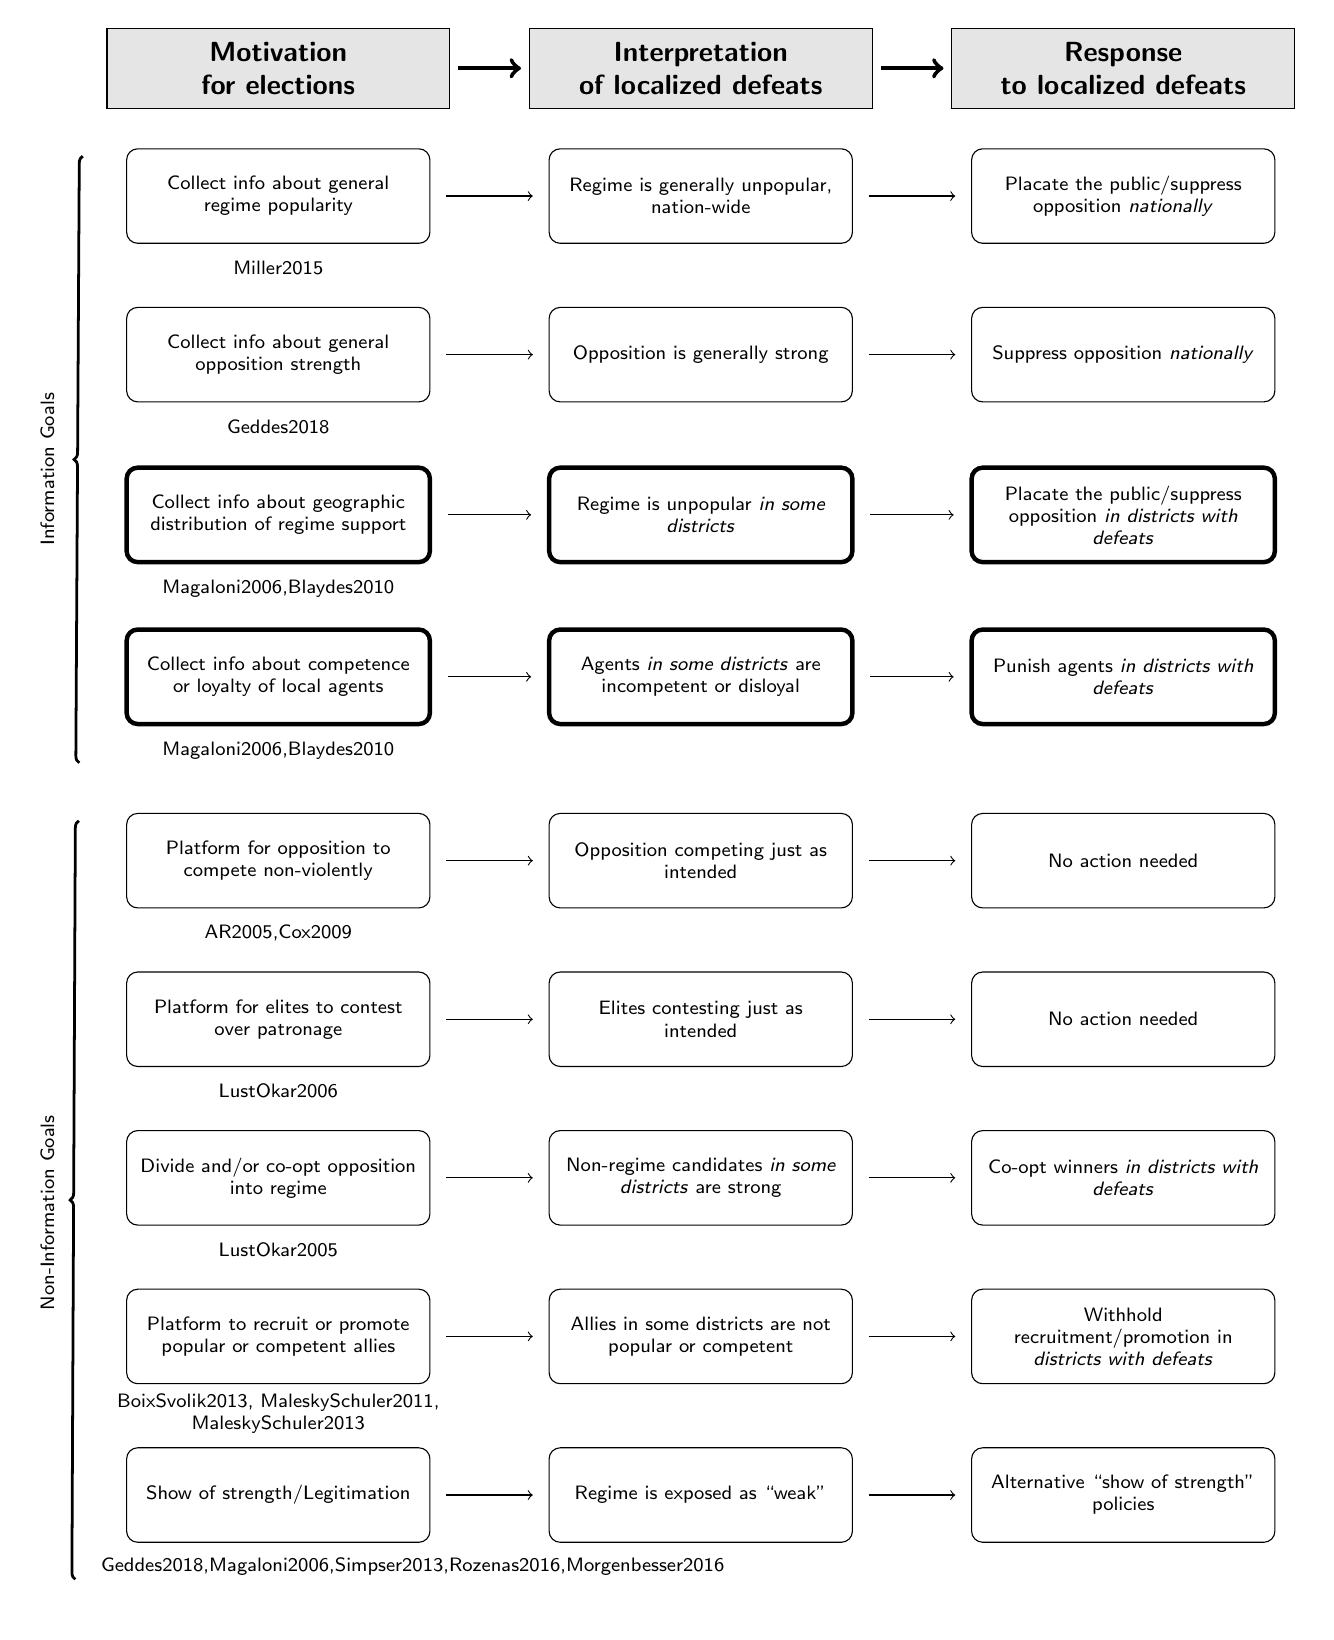
\begin{tikzpicture}
[node distance = 1cm, auto,font=\footnotesize,
% STYLES
every node/.style={node distance=3cm},
% The title style is used to draw the main title
title/.style={rectangle, draw, fill=black!10, inner sep=5pt, text width=4cm, text badly centered, minimum height=1cm, font=\bfseries\footnotesize\sffamily},
% The subtitle style is used to draw the title below main title
subtitle/.style={rectangle, inner sep= 2pt, minimum height=.5cm, node distance=0.25cm, text width=4.5cm, text badly centered, font=\scriptsize\sffamily},
% The theory style is used to draw nodes for each theory
theory/.style={rectangle, rounded corners, draw, minimum height=1.2cm, inner sep= 5pt, text width=3.5cm, node distance=0.25cm, text badly centered, font=\scriptsize\sffamily}]

%%%% Top nodes %%%%
\node [title] (interpretation) {Interpretation\\of localized defeats};
\node [title, left=1cm of interpretation] (intention) {Motivation\\for elections};
\node [title, right=1cm of interpretation] (response) {Response\\to localized defeats};

%% Top nodes subtitle

% Intention
%\node [subtitle, below=0.2cm of intention] (sub-intention) {for\\
%	authoritarian elections};

% Interpretation
%\node [subtitle, below=0.2cm of interpretation] (sub-interpretation) {of\\
%	localized defeats};

% Response
%\node [subtitle, below=0.2cm of response] (sub-response) {to\\
%	localized defeats};

%%%% Theory nodes %%%%
% B1
\node [theory, below=0.5cm of intention] (B1-intention) {Collect info about general regime popularity};
\node [subtitle, below=0.05cm of B1-intention] (B1-sub-intention) {\citep{Miller2015}};

\node [theory, below=0.5cm of interpretation] (B1-interpretation) {Regime is generally unpopular, nation-wide};
\node [subtitle, below=0.05cm of B1-interpretation] (B1-sub-interpretation) {};

\node [theory, below=0.5cm of response] (B1-response) {Placate the public/suppress opposition \textsl{nationally}};
\node [subtitle, below=0.05cm of B1-response] (B1-sub-response) {};

% B2
\node [theory, below=0.8cm of B1-intention] (B2-intention) {Collect info about general opposition strength};
\node [subtitle, below=0.05cm of B2-intention] (B2-sub-intention) {\citep{Geddes2018}};

\node [theory, below=0.8cm of B1-interpretation] (B2-interpretation) {Opposition is generally strong};
\node [subtitle, below=0.05cm of B2-interpretation] (B2-sub-interpretation) {};

\node [theory, below=0.8cm of B1-response] (B2-response) {Suppress opposition \textsl{nationally}};
\node [subtitle, below=0.05cm of B2-response] (B2-sub-response) {};

% B3
\node [theory, below=0.8cm of B2-intention, ultra thick] (B3-intention) {Collect info about geographic distribution of regime support};
\node [subtitle, below=0.05cm of B3-intention] (B3-sub-intention) {\citep{Magaloni2006,Blaydes2010}};

\node [theory, below=0.8cm of B2-interpretation, ultra thick] (B3-interpretation) {Regime is unpopular \textsl{in some districts}};
\node [subtitle, below=0.05cm of B3-interpretation] (B3-sub-interpretation) {};

\node [theory, below=0.8cm of B2-response, ultra thick] (B3-response) {Placate the public/suppress opposition \textsl{in districts with defeats}};
\node [subtitle, below=0.05cm of B3-response] (B3-sub-response) {};

% B4
\node [theory, below=0.8cm of B3-intention, ultra thick] (B4-intention) {Collect info about competence or loyalty of local agents};
\node [subtitle, below=0.05cm of B4-intention] (B4-sub-intention) {\citep{Magaloni2006,Blaydes2010}};

\node [theory, below=0.8cm of B3-interpretation, ultra thick] (B4-interpretation) {Agents \textsl{in some districts} are incompetent or disloyal};
\node [subtitle, below=0.05cm of B4-interpretation] (B4-sub-interpretation) {};

\node [theory, below=0.8cm of B3-response, ultra thick] (B4-response) {Punish agents \textsl{in districts with defeats}};
\node [subtitle, below=0.05cm of B4-response] (B4-sub-response) {};

% A1
\node [theory, below=1.1cm of B4-intention] (A1-intention) {Platform for opposition to compete non-violently};
\node [subtitle, below=0.05cm of A1-intention] (A1-sub-intention) {\citep{AR2005,Cox2009}};

\node [theory, below=1.1cm of B4-interpretation] (A1-interpretation) {Opposition competing just as intended};
\node [subtitle, below=0.05cm of A1-interpretation] (A1-sub-interpretation) {};

\node [theory, below=1.1cm of B4-response] (A1-response) {No action needed};
\node [subtitle, below=0.05cm of A1-response] (A1-sub-response) {};

% A2
\node [theory, below=0.8cm of A1-intention] (A2-intention) {Platform for elites to contest over patronage};
\node [subtitle, below=0.05cm of A2-intention] (A2-sub-intention) {\citep{LustOkar2006}};

\node [theory, below=0.8cm of A1-interpretation] (A2-interpretation) {Elites contesting just as intended};
\node [subtitle, below=0.05cm of A2-interpretation] (A2-sub-interpretation) {};

\node [theory, below=0.8cm of A1-response] (A2-response) {No action needed};
\node [subtitle, below=0.05cm of A2-response] (A2-sub-response) {};

% C1
\node [theory, below=0.8cm of A2-intention] (C1-intention) {Divide and/or co-opt opposition into regime};
\node [subtitle, below=0.05cm of C1-intention] (C1-sub-intention) {\citep{LustOkar2005}};

\node [theory, below=0.8cm of A2-interpretation] (C1-interpretation) {Non-regime candidates \textsl{in some districts} are strong};
\node [subtitle, below=0.05cm of C1-interpretation] (C1-sub-interpretation) {};

\node [theory, below=0.8cm of A2-response] (C1-response) {Co-opt winners \textsl{in districts with defeats}};
\node [subtitle, below=0.05cm of C1-response] (C1-sub-response) {};

% C2
\node [theory, below=0.8cm of C1-intention] (C2-intention) {Platform to recruit or promote popular or competent allies};
\node [subtitle, below=0.05cm of C2-intention] (C2-sub-intention) {\citep{BoixSvolik2013, MaleskySchuler2011, MaleskySchuler2013}};

\node [theory, below=0.8cm of C1-interpretation] (C2-interpretation) {Allies in some districts are not popular or competent};
\node [subtitle, below=0.05cm of C2-interpretation] (C2-sub-interpretation) {};

\node [theory, below=0.8cm of C1-response] (C2-response) {Withhold recruitment/promotion in \textit{districts with defeats}};
\node [subtitle, below=0.05cm of C2-response] (C2-sub-response) {};

% D1
\node [theory, below=0.8cm of C2-intention] (D1-intention) {Show of strength/Legitimation};
\node [subtitle, below=0.05cm of D1-intention] (D1-sub-intention) {\citep{Geddes2018,Magaloni2006,Simpser2013,Rozenas2016,Morgenbesser2016}};

\node [theory, below=0.8cm of C2-interpretation] (D1-interpretation) {Regime is exposed as ``weak''};
\node [subtitle, below=0.05cm of D1-interpretation] (D1-sub-interpretation) {};

\node [theory, below=0.8cm of C2-response] (D1-response) {Alternative ``show of strength'' policies};
\node [subtitle, below=0.05cm of D1-response] (D1-sub-response) {};

%%%% Side theory category nodes %%%%

% B
\node [subtitle, left=1cm of B1-intention.north west, rotate=90, text width = 8cm] (information) {Information Goals};

\draw [decorate,decoration=brace, line width=1pt] 
([xshift=-0.2cm, yshift=0.1cm]B4-sub-intention.south west) -- ([xshift=-0.55cm, yshift=-0.1cm]B1-intention.north west);

% A, C and D together
\node [subtitle, left=1cm of A1-intention.north west, rotate=90, text width = 10cm] (non-information) {Non-Information Goals};

\draw [decorate,decoration=brace, line width=1pt] 
([xshift=-0.25cm, yshift=0.1cm]D1-sub-intention.south west) -- ([xshift=-0.6cm, yshift=-0.1cm]A1-intention.north west);

%% A
%\node [subtitle, left=0.6cm of A1-intention.north west, rotate=90, text width = 4.4cm] (power-sharing) {``Platform''/``Power-sharing''};
%
%\draw [decorate,decoration=brace, line width=1pt] 
%([xshift=-0.2cm, yshift=0.1cm]A2-sub-intention.south west) -- ([xshift=-0.2cm, yshift=-0.1cm]A1-intention.north west);
%
%% C
%\node [subtitle, left=0.6cm of C1-intention.north west, rotate=90, text width = 1.9cm] (co-optation) {``Co-optation''};
%
%\draw [decorate,decoration=brace, line width=1pt] 
%([xshift=-0.2cm, yshift=0.1cm]C2-sub-intention.south west) -- ([xshift=-0.2cm, yshift=-0.1cm]C1-intention.north west);
%
%% D
%\node [subtitle, left=0.6cm of D1-intention.north west, rotate=90, text width = 2cm] (show-of-strength) {``Demonstration''};
%
%\draw [decorate,decoration=brace, line width=1pt] 
%([xshift=-0.2cm, yshift=0.1cm]D1-sub-intention.south west) -- ([xshift=-0.2cm, yshift=-0.1cm]D1-intention.north west);


%%%%%%%%%%%%%%%%

% Draw the links between forces
\path[->,ultra thick, shorten >=.1cm, shorten <=.1cm] 
(intention) edge (interpretation)
(interpretation) edge (response);

\path[->, shorten >=.2cm, shorten <=.2cm] 
(A1-intention) edge (A1-interpretation)
(A1-interpretation) edge (A1-response);

\path[->, shorten >=.2cm, shorten <=.2cm] 
(A2-intention) edge (A2-interpretation)
(A2-interpretation) edge (A2-response);

\path[->, shorten >=.2cm, shorten <=.2cm] 
(B1-intention) edge (B1-interpretation)
(B1-interpretation) edge (B1-response);

\path[->, shorten >=.2cm, shorten <=.2cm] 
(B2-intention) edge (B2-interpretation)
(B2-interpretation) edge (B2-response);

\path[->, shorten >=.2cm, shorten <=.2cm] 
(B3-intention) edge (B3-interpretation)
(B3-interpretation) edge (B3-response);

\path[->, shorten >=.2cm, shorten <=.2cm] 
(B4-intention) edge (B4-interpretation)
(B4-interpretation) edge (B4-response);

\path[->, shorten >=.2cm, shorten <=.2cm] 
(C1-intention) edge (C1-interpretation)
(C1-interpretation) edge (C1-response);

\path[->, shorten >=.2cm, shorten <=.2cm] 
(C2-intention) edge (C2-interpretation)
(C2-interpretation) edge (C2-response);

\path[->, shorten >=.2cm, shorten <=.2cm] 
(D1-intention) edge (D1-interpretation)
(D1-interpretation) edge (D1-response);


\end{tikzpicture} 
\caption{Key theories of authoritarian elections and their predictions about how regime leaders perceive and respond to localized defeats. Two theories most relevant to the Vietnam case are highlighted with bold borders.}
\label{fig:Theory}
\end{figure}


\subsection{The CPV's Response to Central Candidate Defeats}
\label{sec:vietnam_local_defeat}

In the case of Vietnam, what the CPV does in response to the defeats of central candidates in the VNA elections are especially useful in identifying how the party perceives these defeats and consequently what informational goal it had when holding these elections. The reason is that, due to the highly institutionalized and structured nature of Vietnamese politics, the scope of possible actions that the CPV could take following an election is so limited that it would not be able to react to all the incoming information without one reaction compromising the effect of another.

Specifically, if the regime has intended to use the VNA elections to gather information about the distribution of regime popularity, it would see defeats of central candidates as indicators for provinces with faltering public support. The appropriate reaction to this information would be to give the public some sort of concession, which would require an \textit{increase} in central transfers from Hanoi to those provinces. In Vietnam, because most provinces spend more money than it can raise, central transfers are indispensable for local governance, particularly for the provision of public goods. By increasing central transfers, the party enables the provinces to invest in programs that benefits the public, which is the most straightforward thing it can do to bolster regime support .\fnote{Not every regime would see such placation strategy as appropriate for areas with low regime support. As \citet{Magaloni2006} and \citet{Blaydes2010} find in their studies of Mexico and Egypt, the ruling parties do the opposite i.e. cutting transfers to areas with lower ruling party vote share. The difference in context is that no organized opposition exists in Vietnam, which means that central candidate defeats reflect only dissatisfaction towards the CPV and not affinity to any particular opposition party. In addition, even in areas with these localized defeats the absolute level of support for the regime is still sufficiently high, such that a sweeping ``punishment regime'' \citep{Magaloni2006} would hurt regime supporters more than it punishes dissidents.  Cross-national evidence by \citet{Miller2015} seems to suggest that authoritarian regimes generally prefer placation strategies.}

On the other hand, if the CPV has used elections to evaluate province-level officials, the defeats would reveal the identity of provincial leaders who are too incompetent or too independent. The CPV should then punish the officials in question with a \textit{decrease} in central transfers. Like in many other authoritarian regimes, in Vietnam corruption opportunity may be seen as a form of compensation for lower-level officials \citep{Darden2008}. Cutting central transfers reduces the scope for corruption and thus directly affects their income. In addition, it also limits these officials' power by reducing their ability to distribute rent further downwards.

For changes in central transfers to reveal the CPV's interpretation of central candidate defeats, it is not necessary that budget adjustments serve as the primary policy instrument for placating the public or punishing regime agents. As long as each goal requires central transfers to be adjusted in a different direction, observing the direction in which central transfers get adjusted would reveal the CPV's preference between these two goals. Indeed, in this case, increasing central transfers would help appease the public, but would also give local officials some means with which to enrich themselves. Similarly, decreasing central transfers would punish local officials but also deepen resentment among local citizens. In other words, evidence that the CPV altered the flow of transfers to provinces with central candidate defeats in any direction would be sufficient to confirm that it had chosen to listen to one signal and to ignore the other.

\section{Empirical Design}
\label{sec:methods}

To analyze whether the CPV increased or decreased central transfers to provinces where localized defeats had happened, I apply several different panel data methods on cases of close defeats or victories by central candidates to identify the effect of these localized defeats on the amount of central transfer a province received. Identification is achieved by comparing changes in the amount of transfers received prior before and after the election year, between provinces that experienced defeats and provinces that did not. 

I focus my analysis on changes in central transfers before and after the most recent VNA elections, which took place in April 2016. The 2016 elections offer an unprecedented opportunity to conduct such analysis for two main reasons. Firstly, as budget data for Vietnam is only available from 2004 onward, focusing on the most recent election allows for a sufficiently long pre-treatment period of roughly 13 years. The longer the pre-treatment period, the more likely it is that panel data methods can arrive at a credible estimate of the true treatment effects. Secondly and more importantly, the CPV has only released vote shares for defeated candidates starting from the 2016 elections. In contrast, losers in the 2011 and 2007 elections were listed by names only. This means that, for the 2016 elections but not for the 2011 and 2007 elections, I am able to identify central candidates whose defeats were narrow enough that they can be plausibly considered as similar to those who have won. Following the regression-discontinuity logic, this rules out potential confounding factors that could result from candidate-level differences between central winners and losers, allowing the identified treatment effect to be attributable to the result alone. For these two reasons, focusing on the 2016 elections offers the most causally rigorous analysis that could be achieved with given data. In the spirit of generalizability, however, in the Online Appendix I show that a slightly less conservative analysis of the 2011 and 2007 elections also yield consistent results.

\subsection{Estimation Methods}
\label{sec:methods_estimation}
I employ in conjunction three different estimation and inference methods. First of all, I leverage the panel structure of the data with a linear fixed effects model:

\begin{equation}
\Delta Y_{it} = \beta D_{it} + \omega T_{i} + \gamma X_{it} + \lambda_i + \delta_t + \epsilon_{it} \label{eq:FE}
\end{equation}
where $\Delta Y_{it}$ is the log of the first difference in net central transfers for province $i$ at time $t$ i.e. $\Delta Y_{it} = \log(Y_{it} - Y_{i, t-1})$ and $X_{it}$ is a vector of time-varying covariates. $T_{i}$ takes the value of 1 for every province that experienced localized defeat in 2017 and 0 otherwise, and does so for every year in the sample. Depending on whether the model seeks to estimate the \textit{instantaneous} effect that occurs in the year after, or the \textit{persistent} effect that manifests in all post-election years, $D_{it} = T_{i}$ for $t=2017$ or $t\geq2017$, and is  $0$ otherwise.\fnote{$D_{it}$ is ``lagged'' by one year for the fact that budget allocation decisions are made at the beginning of each year, such that the effect of the 2016 election only begins to manifest in 2017.} Here, $\lambda_i$ and $\delta_t$ are province and time fixed effects. For all analyses, $t \in \{2012, \ldots, 2018\}$ to exclude the years before the previous election.

Whereas standard fixed effects models are generalization of the difference-in-difference framework, the use of first-differenced outcome here generalizes my model to the triple differences method. Specifically, by allowing potential outcomes to be framed in terms of changes compared to previous years, the model can account for differences in pre-treatment trends across treated and control provinces. This is because whereas the standard difference-in-difference compares difference in pre- and post-treatment means across treatment groups, my model would also subtract away from this difference the year-to-year changes in outcomes, which may be different for each group. It thus relaxes the assumption of parallel trends to one of linear trends.

Secondly, I conduct an additional regression discontinuity analysis using the local randomization approach by \citet{CattaneoTitiunik2015}. This method offers a solution for the small sample size, which otherwise would not only cause problems with inference for the fixed effects methods but also prevent the standard regression discontinuity method. The intuition behind it is that, for a small enough window around the treatment assignment threshold, any unit's treatment status can be considered a coin flip from an as-if randomized experiment. This interpretation then allows for exact randomization-based inference methods, which is more appropriate for finite samples. Specifically, I use independent coin flips to re-randomize $10,000$ times the election outcomes for each central candidate whose vote margin lies within the window, aggregate the resulting candidate-level treatment status vectors to obtain province-level treatment status vectors, estimate new treatment effects (using Model \ref{eq:FE}), and then compare the original effect with the distribution of these re-randomized treatment effects.

Finally, to eliminate the problem of dynamic causality \citep{ImaiKim2019}, which arises out of the interdependence between central transfers in pre-election years (past outcomes), central transfers in post-election years (future outcomes), and election results (treatment), I also implement a generalized synthetic control analysis \citep{Xu2017gsynth}. This method improves on the original synthetic control method \citep{Abadie2010} by allowing for easy calculation of treatment effects across multiple treated units. The fundamental intuition remains unchanged: by using a synthetic control made from a weighted average of control units to be identical to treated units in terms of pre-treatment outcomes, it is possible for the treated effect to be free from the influence of pre-treatment differences. Additionally, because it neutralizes the effect of previous treatment, the generalized synthetic control method accepts a much longer panel without suffering from the confounding effect of central candidate defeats in previous elections. This allow my synthetic control to take into account outcome values from 2004 to 2018, as well as a set of time-varying covariates, specifically each province's histories of central candidate defeats in previous elections and its lagged total revenue.

\subsection{Identifying Close Defeats}
\label{sec:methods_sample}

For all these methods, a key empirical problem is that provinces that did experience these defeats may be different from those that did not in ways that matter for central transfers. \citet{MaleskySchuler2011} already show that provinces where defeats happened tend to be more independent, in the sense that they raise more income on their own and are located further from Hanoi. My argument's very premise also suggests that they may have dissatisfied voters or low-quality bureaucrats. At the candidate level, some candidates are also less likely to lose than others: even the country's highest leaders run in the VNA elections, but the CPV is not going to allow them to lose. The provinces these leaders are allocated to can be expected to have lower chance of suffering defeats. 

Drawing insights from the matching methods and the regression-discontinuity design, I restrict the analysis to provinces where at least one central candidate has won or lost with a margin of no more 10 percentage points.\fnote{Margins for winning candidates are in reference to whichever is higher between the best-performing losing candidates' vote shares or the 50 percent threshold. A similar procedure applies to losing candidates} I use the 10 percentage point margin based on the observation that it is officially considered a low winning threshold by the CPV, such that winning candidates with vote shares below 60 percent had to formally self-criticize \citep{MaleskySchuler2011}. I also drop the capital Hanoi and the biggest municipality Ho Chi Minh City. These steps remove all the provinces where central candidates's \textit{a posteriori} vote share is so large that their \textit{a priori} probability of losing can be inferred to be zero, and leave a set of control group similar enough to the treated group.

Another approach is to achieve as-if randomization at the candidate level. Following \citet{CattaneoTitiunik2015}, I conduct a grid search to identify the upper and lower vote margin boundaries that would produce the largest window within which central candidates who lost and who won are statistically indistinguishable in terms of every pre-treatment candidate-level and district-level characteristics.\fnote{Specifically, I  increment each boundary by $0.25$ at a time to generate a grid of possible windows. For each window, I test the sharp null hypothesis of no treatment effects on each of the chosen characteristics using the ATE test statistic, and reject any window for which the minimum p-value of these tests is above 0.15. The candidate-level characteristics are age, gender, party membership, party history, education, political power (operationalized following \citet{MaleskySchuler2011}), and the district-level characteristics are number of candidates and number of seats.} The resulting window is found to be $(-11.25, 7.75)$. Since the fates of central candidates whose vote shares fell within this window can be assumed to be generated by chance, it is possible to conduct inference through independent re-randomization. 

The two approaches produce two slightly different samples, but both achieve remarkable balance. Table \ref{tab:balance} shows the balance between control provinces (without central candidate defeats) and treated provinces (with central candidate defeats) across a number of relevant covariates, all of which are measured in 2015. To provide context, the difference in means between the two groups are standardized by the pooled standard deviation. For both samples, the difference between treatment and control means is subjected to both a randomization-inference based and a standard OLS-based hypothesis test. The results show that treated and control provinces in the first sample are similar except for a few variables. The second sample, even though constructed to achieve balance only at the candidate and district levels, displays perfect balance when aggregated to the province level. 

I use the first sample for my linear fixed effects model, and the second for the local randomization regression discontinuity analysis. Because the synthetic control achieves balance on pre-treatment outcomes by design, I construct it from a relaxed version of the first sample, which includes provinces with close victories or defeats in not only the 2016 but also the 2011 and 2007 elections.


\begin{landscape}\begin{table}[!h]

\caption{\label{tab:balance}Balance between control and treatment provinces based on 2015 data}
\centering
\resizebox{\linewidth}{!}{
\begin{tabular}{>{\raggedright\arraybackslash}p{14em}>{\raggedleft\arraybackslash}p{4.1em}>{\raggedleft\arraybackslash}p{4.1em}>{\centering\arraybackslash}p{4.1em}>{\centering\arraybackslash}p{4.1em}>{\centering\arraybackslash}p{4.1em}>{\raggedleft\arraybackslash}p{4.1em}>{\raggedleft\arraybackslash}p{4.1em}>{\centering\arraybackslash}p{4.1em}>{\centering\arraybackslash}p{4.1em}>{\centering\arraybackslash}p{4.1em}}
\toprule
\multicolumn{1}{c}{ } & \multicolumn{5}{c}{Linear Fixed Effects Sample} & \multicolumn{5}{c}{Local Randomization RDD Sample} \\
\cmidrule(l{3pt}r{3pt}){2-6} \cmidrule(l{3pt}r{3pt}){7-11}
\multicolumn{1}{>{\centering\arraybackslash}p{14em}}{ } & \multicolumn{1}{>{\centering\arraybackslash}p{4.1em}}{Control Mean ($N = 9$)} & \multicolumn{1}{>{\centering\arraybackslash}p{4.1em}}{Treated Mean ($N = 5$)} & \multicolumn{1}{>{\centering\arraybackslash}p{4.1em}}{Std. Diff. in Means} & \multicolumn{1}{>{\centering\arraybackslash}p{4.1em}}{RI p-value} & \multicolumn{1}{>{\centering\arraybackslash}p{4.1em}}{OLS p-value} & \multicolumn{1}{>{\centering\arraybackslash}p{4.1em}}{Control Mean ($N = 11$)} & \multicolumn{1}{>{\centering\arraybackslash}p{4.1em}}{Treated Mean ($N = 4$)} & \multicolumn{1}{>{\centering\arraybackslash}p{4.1em}}{Std. Diff. in Means} & \multicolumn{1}{>{\centering\arraybackslash}p{4.1em}}{RI p-value} & \multicolumn{1}{>{\centering\arraybackslash}p{4.1em}}{OLS p-value}\\
\midrule
\addlinespace[0.3em]
\multicolumn{11}{l}{\textbf{Budget}}\\
\hspace{1em}Budget Revenue (Billions of VND) & 3087.7 & 3187.2 & 0.06 & 0.92 & 0.94 & 5576.0 & 3753.2 & -0.20 & 0.92 & 0.71\\
\hspace{1em}Budget Expenditure (Billions of VND) & 5082.6 & 4840.6 & -0.14 & 0.78 & 0.78 & 5523.6 & 4942.5 & -0.26 & 0.69 & 0.64\\
\addlinespace[0.3em]
\multicolumn{11}{l}{\textbf{Election}}\\
\hspace{1em}Number of Seats & 7.4 & 6.8 & -0.57 & 0.39 & 0.29 & 7.5 & 6.8 & -0.71 & 0.16 & 0.23\\
\hspace{1em}Number of Candidates & 13.0 & 12.4 & -0.32 & 0.68 & 0.60 & 13.4 & 11.8 & -0.87 & 0.13 & 0.17\\
\hspace{1em}Number of Central Candidates & 3.1 & 2.6 & -0.65 & 0.34 & 0.22 & 3.2 & 2.5 & -0.91 & 0.07 & 0.13\\
\addlinespace[0.3em]
\multicolumn{11}{l}{\textbf{Structural Condition}}\\
\hspace{1em}Surface Area (Thousands Km$^2$) & 4720.8 & 3100.2 & -0.48 & 0.31 & 0.33 & 4408.5 & 3047.4 & -0.44 & 0.42 & 0.43\\
\hspace{1em}Population (Thousands) & 1273.6 & 1234.2 & -0.07 & 0.85 & 0.88 & 1338.2 & 1215.1 & -0.24 & 0.64 & 0.67\\
\hspace{1em}Population Density (Thousands/Km$^2$) & 399.7 & 479.8 & 0.23 & 0.65 & 0.66 & 428.7 & 500.8 & 0.22 & 0.68 & 0.70\\
\addlinespace[0.3em]
\multicolumn{11}{l}{\textbf{Economic}}\\
\hspace{1em}Provincial GDP (Billions of VND) & 45369.4 & 42131.1 & -0.15 & 0.76 & 0.77 & 58482.0 & 43129.7 & -0.31 & 0.64 & 0.56\\
\hspace{1em}Average Monthly Income (Thousands of VND) & 2102.9 & 2159.4 & 0.13 & 0.85 & 0.80 & 2237.1 & 2221.0 & -0.03 & 0.96 & 0.96\\
\hspace{1em}Employment Rate Among >15yo Population ($\%$) & 60.7 & 56.4 & -0.95 & 0.06 & 0.09 & 60.2 & 57.5 & -0.56 & 0.30 & 0.32\\
\hspace{1em}Share of Agriculture Land ($\%$) & 44.9 & 62.6 & 0.81 & 0.14 & 0.16 & 49.1 & 62.2 & 0.60 & 0.31 & 0.33\\
\addlinespace[0.3em]
\multicolumn{11}{l}{\textbf{Public Goods}}\\
\hspace{1em}Infant (<5yo) Mortality Rate (\textperthousand) & 23.2 & 18.5 & -0.38 & 0.52 & 0.42 & 22.0 & 18.2 & -0.33 & 0.68 & 0.54\\
\hspace{1em}Number of Beds in Public Hospitals & 3646.3 & 3324.0 & -0.29 & 0.67 & 0.66 & 3516.1 & 3442.2 & -0.07 & 0.93 & 0.92\\
\hspace{1em}Number of Schools & 433.9 & 377.4 & -0.39 & 0.47 & 0.45 & 418.5 & 359.8 & -0.42 & 0.50 & 0.46\\
\hspace{1em}Number of Primary Schools & 239.0 & 235.8 & -0.04 & 0.98 & 0.95 & 235.7 & 220.5 & -0.17 & 0.79 & 0.76\\
\bottomrule
\end{tabular}}
\end{table}
\end{landscape}


\section{Results}
\label{sec:results}

% Table created by stargazer v.5.2.2 by Marek Hlavac, Harvard University. E-mail: hlavac at fas.harvard.edu
% Date and time: Wed, Feb 19, 2020 - 3:24:00 AM
\begin{table}[!htbp] \centering 
  \caption{Estimated treatment effects of localized defeats on central transfers from linear fixed effects models} 
  \label{tab:lfe_main} 
\begin{tabular}{@{\extracolsep{5pt}}lcccccc} 
\\[-1.8ex]\hline 
\hline \\[-1.8ex] 
 & \multicolumn{3}{c}{Instantaneous Effect} & \multicolumn{3}{c}{Persistent Effect} \\ 
\\[-1.8ex] & (1) & (2) & (3) & (4) & (5) & (6)\\ 
\hline \\[-1.8ex] 
 Treatment Effect & 9.093$^{**}$ & 9.104$^{*}$ & 9.093$^{**}$ & 10.385$^{***}$ & 10.376$^{**}$ & 10.385$^{***}$ \\ 
  & (4.580) & (4.684) & (4.223) & (4.026) & (4.229) & (3.769) \\ 
 \hline \\[-1.8ex] 
Election Competitiveness &  &  & Yes &  &  & Yes \\ 
Time-variant Covariates &  & Yes &  &  & Yes &  \\ 
Province FEs & Yes & Yes &  & Yes & Yes &  \\ 
Year FEs & Yes & Yes & Yes & Yes & Yes & Yes \\ 
\hline \\[-1.8ex] 
N & 70 & 70 & 70 & 84 & 84 & 84 \\ 
R$^{2}$ & 0.604 & 0.604 & 0.439 & 0.510 & 0.512 & 0.414 \\ 
\hline 
\hline \\[-1.8ex] 
\multicolumn{7}{l}{$^{*}$p $<$ .1; $^{**}$p $<$ .05; $^{***}$p $<$ .01} \\ 
\end{tabular} 
\end{table} 


Table \ref{tab:lfe_main} shows the main results from the linear fixed effects model in Section \ref{sec:methods_estimation} under different model specifications. The treatment effect estimates are positive and significant across specifications, and are relatively stable. Given that the outcome variable is the log of first-differenced net transfers, the effect magnitude would be best understood as a percentage of the average absolute annual change in net transfers between non-election years. For example, if net transfers to a province have been growing at an average rate of $100$ billion VND (approx. 4.3 million USD) per year, then a localized defeat would see the province' net transfers in 2017 increased by an additional $13$ billion VND (approx. $560,000$ USD), as indicated in the first three columns of Table \ref{tab:lfe_main}. When averaged over both 2017 and 2018, the treatment effect is slightly bigger, suggesting that the effect of localized defeats on net transfers accumulates over a long duration rather than going away.\fnote{Among the provinces in the sample, Tien Giang experienced the smallest average change in net transfers -- approximately $56$ billion VND (2.4 million USD) per year, whereas Binh Duong experienced the largest -- approximately $2575$ billion VND (111 million USD) per year. Because Binh Duong contributes more to the national budget than it takes from central transfers, the change actually means that that it gets to keep more of its revenues. The estimated effect translates to roughly $7$ billion VND ($300,000$ USD) for Tien Giang and $335$ billion VND (14.4 million USD) for Binh Duong. For perspective, average total expenditure is $5,500$ billion VND (237 million USD) for Tien Giang and $11,100$ billion VND (479 million USD) for Binh Duong.}

To allay concerns about lack of exogeneity, Figure \ref{fig:lfe_placebo} plots the first three estimates in Table \ref{tab:lfe_main} against three placebo treatment effects. The placebo treatment effects are estimated by moving the treatment indicators backward in time as if the election has happened earlier than it actually did. In particular, I estimate three placebo effects for 2013, 2014, and 2015. Because the election could not have left any effect on planned budgets before it took place, the true treatment effects should be zero for these years, and any measured difference between treated and untreated provinces would only reflect imbalance in the data. The results in Figure \ref{fig:lfe_placebo} reassuringly show no such difference. Only the 2014 placebo effect is estimated to be far from zero, but even then it is statistically insignificant.

\begin{figure}[!htbp]
	\centering
	\includegraphics[width=\textwidth]{figure/200205_lfe_placebo.png}
	\captionsetup{singlelinecheck=off}
	\caption[Estimated placebo linear fixed effects treatment effects]{Estimates of instantaneous treatment effects using linear fixed effects models. The error bars show 95\% confidence intervals.}
	\label{fig:lfe_placebo}
\end{figure}

Figure \ref{fig:rdd_placebo} presents the results from an analysis based on the local randomization interpretation of the regression discontinuity framework. Since this analysis uses a randomization procedure that does not rely on large sample asymptotics, its inferences are less subjected to the small sample concerns that may have cast doubt on the previous results. Reassuringly, the results show the treatment effect to be statistically similar to those found in Table \ref{tab:lfe_main}. Specifically, the estimated effect of losing central candidates is estimated to be a 10\% addition to a province's annual change in central transfers. The placebo results suggest that imbalance between treated and untreated provinces are small and close to zero. Similar to Figure \ref{fig:lfe_placebo}, a negative but statistically insignificant difference is detected for the 2014 placebo. 

\begin{figure}[!htbp]
	\centering
	\includegraphics[width=\textwidth]{figure/200205_rdd_results.png}
	\captionsetup{singlelinecheck=off}
	\caption[Estimated RDD treatment effects]{Estimates of instantaneous treatment effects for RDD analyses using the local randomization approach. The red lines show the estimated treatment effects, and the gray bars show their randomization distribution. P-values are presented for the treatment effect estimate.}
	\label{fig:rdd_placebo}
\end{figure}

The absence of statistically significant placebo effects in Table \ref{tab:lfe_main} and Figure \ref{fig:rdd_placebo} suggests little threat of dynamic causality. However, to remain as conservative as possible, I conduct an additional analysis using the generalized synthetic control method \citep{Xu2017gsynth} which is particularly effective at addressing dynamic causality. The results, shown in Figure \ref{fig:synth_placebo}, confirm not only a significant and sustained treatment effect for 2017 and 2018, but also the absence of any difference across treated units and the synthetic control in the years prior to the election. The magnitude of the treatment effect is consistent with previous results.

\begin{figure}[!htbp]
	\centering
	\includegraphics[width=\textwidth]{figure/200205_synth_results.png}
	\captionsetup{singlelinecheck=off}
	\caption[Estimated synthetic control treatment effects]{Estimates of treatment effects on net transfers using the generalized synthetic control method. The horizontal dashed line marks the election year.}
	\label{fig:synth_placebo}
\end{figure}

Altogether, the three different analyses present a robust and consistent set of findings, according to which the central government in Vietnam increased the amount of central transfers to provinces that suffered defeats of central candidates in the 2016 election. The resulting treatment effect is statistically and substantively significant across all specifications, and have survived sufficient placebo tests. It lends credibility to the hypothesis that the CPV leadership considered election setbacks as indicators for areas of low regime support, and chose to remedy this problem by increasing central support to these areas.

\section{Additional Evidence}
\label{sec:additional}

Some additional evidence allows us to confidently link the finding of a significant increase in central transfers to provinces with central candidate defeats with the conclusion that the CPV uses elections to identify areas of abnormally low regime support.

\subsection{Effect of Increased Central Transfers}

The argument in Section \ref{sec:vietnam_local_defeat} requires not only that the CPV increased central transfers to areas it observes weaker regime support, but also that it did so to placate the dissatisfied voting public. For this to happen, the increased flow of money should have been spent on public goods that directly benefit citizens. In addition, there should have been no significant re-allocation of expenditure from items that benefit local officials to those that benefit citizens, or else the net increase in central transfers would still mask a direct punishment to provincial leaders. 

I find evidence to support both propositions by looking at two line items in each province's budget: development spending, which consists mostly of investment on public projects, and administrative spending, which includes from large procurement orders to recurrent expenses such as salaries, travel reimbursements or even office supplies, most of which directly affect the livelihood of provincial bureaucrats. Straightforwardly, an increase in development spending would be evident of placation towards citizens, whereas cuts in administrative spending would suggest punishment towards provincial officials. Available data confirms the former, but find no evidence for the latter.


% Table created by stargazer v.5.2.2 by Marek Hlavac, Harvard University. E-mail: hlavac at fas.harvard.edu
% Date and time: Wed, Mar 13, 2019 - 02:56:38 AM
\begin{table}[!htbp] \centering 
  \caption{Estimated treatment effects on development and administration expenditures from linear fixed effects models} 
  \label{tab:lfe_mech} 
\begin{tabular}{@{\extracolsep{5pt}}lcccccc} 
\\[-1.8ex]\hline 
\hline \\[-1.8ex] 
 & \multicolumn{3}{c}{Development Expenditure} & \multicolumn{3}{c}{Administrative Expenditure} \\ 
\\[-1.8ex] & (1) & (2) & (3) & (4) & (5) & (6)\\ 
\hline \\[-1.8ex] 
 Treatment Effect & 0.558$^{**}$ & 0.542$^{**}$ & 0.558 & 0.302 & 0.293 & 0.302 \\ 
  & (0.260) & (0.251) & (0.478) & (0.181) & (0.177) & (0.202) \\ 
 \hline \\[-1.8ex] 
Election Competitiveness &  &  & Yes &  &  & Yes \\ 
Time-invariant Covariates &  & Yes &  &  & Yes &  \\ 
Province FEs & Yes & Yes &  & Yes & Yes &  \\ 
Year FEs & Yes & Yes & Yes & Yes & Yes & Yes \\ 
\hline \\[-1.8ex] 
N & 60 & 60 & 60 & 60 & 60 & 60 \\ 
R$^{2}$ & 0.847 & 0.861 & 0.397 & 0.598 & 0.623 & 0.412 \\ 
\hline 
\hline \\[-1.8ex] 
\multicolumn{7}{l}{$^{*}$p $<$ .1; $^{**}$p $<$ .05; $^{***}$p $<$ .01} \\ 
\end{tabular} 
\end{table} 


Specifically, Table \ref{tab:lfe_mech} and Figure \ref{fig:synth_rdd_mech} present the above evidence, with the former presenting estimates from linear fixed effects model and the latter showing graphically the results from the local randomization regression discontinuity and generalized synthetic control analyses. There are positive and stable treatment effects on both outcomes, but the effect on development spending is bigger, and is statistically significant in Table \ref{tab:lfe_mech}. Compared to the analyses in Section \ref{sec:methods_estimation}, the only difference is that the linear fixed effects models in this section do not use log-differenced outcome. This is because detailed budget breakdowns are available only for a subset of provinces, and then are sporadically missing for some years. Calculating log-differences would only exacerbate this missingness. This caveat changes the interpretation of the treatment effect's magnitude but does not compromise rigor, as every specification still passes all placebo tests (not shown in the interest of space).

\begin{figure}[!htbp]
	\centering
	\includegraphics[width=\textwidth]{figure/200205_mech_results.png}
	\captionsetup{singlelinecheck=off}
	\caption[Estimated RDD and synthetic control treatment effects]{Estimates of treatment effects on development and administrative expenditure using RDD under the local randomization approach and the generalized synthetic control method. Only effects for 2017 are calculated due to lack of 2018 data.}
	\label{fig:synth_rdd_mech}
\end{figure}

\subsection{Alternative Mechanisms for Increased Central Transfers}

Another plausible criticism is that the increase in downward flow of money, even if being channeled towards public goods, may not reflect a top-down decision to buy off the public, but was instead the result of bottom-up demand. From this perspective, localized defeats led to increased central transfers not because they sent a signal from the provinces to Hanoi, but because each defeated central candidate left a seat for local elites to fill, strengthening the province's representation and bargaining power in the legislature.

It is possible to rule out this alternative explanation by looking at provinces where central candidate defeats did not translate to additional seats for local candidates i.e. cases where central candidates lost because they failed to clear the 50 percent threshold. In the two provinces of Soc Trang and Can Tho where this happened, because the central candidate still outperformed the closest local competitor, neither ended up winning the election, leaving the province with an unfilled seat and no increased representation. 

\begin{figure}[!htbp]
	\centering
	\includegraphics[width=\textwidth]{figure/200205_synth_results_2prov.png}
	\captionsetup{singlelinecheck=off}
	\caption[Individual synthetic control treatment effects]{Individual estimates of treatment effects on central transfers for Soc Trang and Can Tho, estimated using the generalized synthetic control method similar to Table \ref{fig:synth_placebo}.}
	\label{fig:synth_mech}
\end{figure}

Because the generalized synthetic control method allows treatment effects to be extracted for individual units, I show in Figure \ref{fig:synth_mech} that both provinces experienced increased central transfers in 2017 and 2018 when compared to the synthetic control. Although the 95\% confidence intervals are large and cross zero due to insufficient power, the point estimates suggest that both provinces saw large increases in central transfers -- approximately 10\% of previous years' annual change for Soc Trang and nearly 20\% for Can Tho. While this finding is far from conclusive, it does offer some good evidence to dismiss negotiation and bargaining through representation as the primary driver for the main treatment effects.

\subsection{Absence of Other Punishment}

To further confirm that provincial leaders did not receive punishment for central candidate defeats, I use data on the career tracks of top Vietnamese politicians provided by \citet{MaleskyPhan2017} to see whether these defeats have had any impact on their career prospects. The data allows me to identify for all officials who have ever governed in a province -- defined as holding one of the top two provincial leadership positions -- whether they have gone on to hold higher Party or government positions. I conduct this test only on officials who were governing before the 2007 and 2011 elections however, because those governing in 2016 would not have completed their current term.

The data in Table \ref{tab:promo_mech} shows the number of provinces that have had zero, one, or both of its top leaders promoted, separated by treatment status. In case there is shuffling of provincial leadership in the election year, I calculated promotion records for both leaders who are in power \textit{before} and \textit{during} the election year. This would account for both the possibilities that the CPV sees elections as a referendum on either the governing performance or the election management performance of provincial officials. Promotion records are calculated for the entire term i.e. 2006-2010 for those governing in 2005 and 2006, and 2011-2015 for those governing in 2010 and 2011.

% latex table generated in R 3.6.0 by xtable 1.8-4 package
% Tue Jun 18 17:54:55 2019
\begin{table}[ht]
\centering
\begin{tabular}{lcccccccc}
   & \multicolumn{2}{c}{Gov. in 2006} & \multicolumn{2}{c}{Gov. in 2007} & \multicolumn{2}{c}{Gov. in 2010} & \multicolumn{2}{c}{Gov. in 2011} \\
 & $T = 0$ & $T = 1$ & $T = 0$ & $T = 1$ & $T = 0$ & $T = 1$ & $T = 0$ & $T = 1$ \\
 \hline
No Promotion & 1 & 4 & 1 & 4 & 4 & 5 & 2 & 4 \\ 
  1 Promotion & 5 & 2 & 5 & 2 & 3 & 2 & 5 & 2 \\ 
  2 Promotions & 0 & 0 & 0 & 0 & 2 & 1 & 2 & 2 \\ 
   \hline
Fisher Odd Ratio & 0.13 &  & 0.13 &  & 0.50 &  & 0.31 &  \\ 
  Fisher p-value & 0.12 &  & 0.12 &  & 0.40 &  & 0.25 &  \\ 
  \end{tabular}
\caption{Summary of promotion records for the top two leaders in all the provinces in the restricted sample. 
             Promotion records are calculated for leaders who are in power in 2006 (ruling just before the 2007 election), 2007 (in charge of managing the 2007 election),
             2010 (ruling just before the 2011 election), and 2011 (in charge of managing the 2011 election).} 
\label{tab:promo_mech}
\end{table}


Table \ref{tab:promo_mech} shows no significant difference in the frequency of promotion among officials in provinces with and in provinces without central candidate defeats. Where there seems to be a difference, the gap is never big enough for a Fisher's exact test to reject the null hypothesis. This evidence suggests that the top party leadership did not delay the promotion of provincial officials even when central candidate defeats had happened under their jurisdiction.

This finding is consistent with the observation that, unlike in other nondemocratic regimes such as Russia \citep{Myagkov2009}, Vietnam's leaders rely on punishment much more sparingly, reserving demotion or firing only to very serious transgressions. %\fnote{Two illustrative anecdotes suggest that the CPV avoids punishment because it draws attention to disunity within the party, and that it only punishes top officials in case of extreme transgressions. In 2012, when the CPV's highest leadership debated and decided against officially censuring then-PM Nguyen Tan Dung for economic mismanagement, official statements from the Party refers to him only as ``one comrade'' without mentioning any name \citep{voa2012}. Later, in 2017, when the Party's leaders finally decided to punish Ho Chi Minh City's Party Secretary Dinh La Thang and to publicly acknowledge this decision, it was only after mismanagement of PetroVietnam, Vietnam's largest SOE and where Thang had served as chairman between 2009 and 2001, has been found to cost the country close to US\$150 million \citep{BBC2017}.} 
In addition, the CPV only makes major personnel decisions at its Party Congress, which takes place every five year and usually just before an election (presumably so that the election could ratify and legitimize newly appointed leaders). This makes the time lag between one election's outcomes and the next batch of promotion decisions too large for the latter to be useful as punishment for the former.

\section{Discussion and Conclusion}

The thriving literature on authoritarian institutions in general and authoritarian elections in particular has identified a number of governance goals that elections can achieve for authoritarian rulers, many of which center around elections' ability to provide information on variables that dictators cannot access easily. Left unconsidered by this literature, however, is the reality that each authoritarian regime can only seek and receive a limited amount of information from elections, no matter how many different signals these elections can emit. Indeed, dictators seeking too many different types of information risk facing dissonance from potentially conflicting information signals and contradictory policy recommendations. As a result, authoritarian rulers are expected to focus each election towards a limited number of prioritized information goals.

To identify which kind of information each dictator chooses to collect from elections, outside observers may gain significant inferential leverage by paying attention to the dictator's post-election responses when faced with surprising localized defeats. These responses are informative because they are tied to the regime's interpretation of localized defeats, namely what they believe to have caused these defeats; this interpretation in turn must be motivated by the original informational purpose. In other words, dictators see in elections what they seek to see, and react based on what they see.

The case of Vietnam's National Assembly election in 2016 demonstrates this logic. Even though it presides over a highly capable single-party regime, the Communist Party of Vietnam still faces serious information problems, in particular when it comes to knowing where in the country it enjoys weaker public support and who among its high-level agents are less reliable. A close look at the rare defeats of centrally-nominated candidates in the 2016 legislative election shows that the Hanoi leadership can pursue only one type of information through national elections: either it seeks to learn about the geographic distribution of regime popularity and considers such defeats evidence of low support areas, or it hopes to evaluate its agents' performance and attributes the defeats to the incompetence or disloyalty of province-level officials in charge of election management. Each of these interpretations would produce a different policy recommendation, but in this case the two recommendations are diametrically opposite: the first interpretation would call for placating the unhappy public through increased central transfers to provinces where defeats happen, whereas the second would suggest punishing the weak officials by cutting transfers to the same provinces.

A combination of different empirical approaches finds that Vietnam's leaders increased central transfers to provinces they have suffered localized defeats in, thereby confirming that these leaders sought and thus saw in these defeats only signals about regime popularity. Additional evidence further shows that the increased transfers were indeed used towards development expenditure, and were offered without upwards push by elected legislators. This is consistent with the idea that Hanoi used this signal to identify pockets of dissatisfied citizens to placate. Moreover, officials in provinces with defeats did not experience any other form of punishment, suggesting that the Party did not see the results as informative about regime agent competence or loyalty, despite their apparent needs for this information and the election's ability to provide it. 

Precisely because its empirical evidence draws from the case of Vietnam, this paper's findings may contribute significantly to the understanding of authoritarian resilience in other areas of the world. Specifically, if even this strong, highly institutionalized, single-party regime, with all the power needed to consistently command near-perfect election results, still cannot satisfy all its information needs by holding authoritarian elections, then perhaps there really is an upper limit to how much assistance elections and other authoritarian institutions could provide for the dictators of the world. In addition, the Vietnamese regime's decision to prioritize signals about its popularity suggests that autocrats and and do respond to public satisfaction. This echoes other findings in the literature that even formal authoritarian institutions may offer pathways to accountability \citep[e.g.][]{Miller2015,Lorentzen2013}, but calls into questions existing claims that autocrats pay more attention to governing their own subordinates than to keeping citizens content \citep[e.g.][]{Svolik2012}.

More importantly, this paper contributes an empirical framework against which theories of authoritarian institutions could be tested. For the test to work, regime rulers must have only a limited set of post-election responses but also some degree of control over the election process. Even though this applies most particularly to highly institutionalized regimes such as the single-party states of Vietnam, Singapore or China, it may also succeed in a broad range of other authoritarian regimes where the lack of discretion over post-election responses may have been placed by lack of capacity rather than institutionalization.

\newpage
\inputencoding{utf8}
\printbibliography[heading=bibintoc]

\end{document}


